\documentclass[tikz, border=10pt]{standalone}
\usepackage{tikz}
\usetikzlibrary{arrows.meta, positioning, shapes.geometric, calc}

\begin{document}
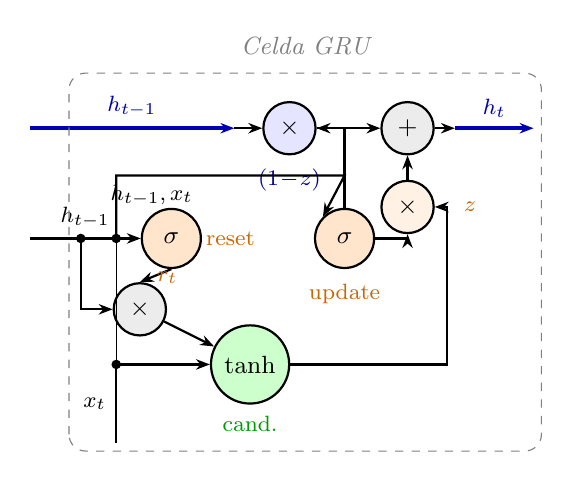
\begin{tikzpicture}[
    gate/.style={draw, circle, minimum size=0.75cm, thick, fill=orange!20},
    op/.style={draw, circle, minimum size=0.65cm, thick, fill=gray!15},
    tanh/.style={draw, circle, minimum size=0.75cm, thick, fill=green!20},
    arr/.style={-{Stealth[length=5pt]}, thick},
    font=\small,
    lbl/.style={font=\footnotesize}
]

% ---- h_t output line (top, blue) ----
% h_t = (1-z)·h_{t-1} + z·h̃_t
\draw[arr, line width=1.4pt, blue!70!black]
    (-0.8, 3.2) -- node[above, lbl, blue!70!black]{$h_{t-1}$} (1.8, 3.2);
\draw[arr, line width=1.4pt, blue!70!black]
    (4.6, 3.2) -- node[above, lbl, blue!70!black]{$h_t$} (5.6, 3.2);

% Operations on h_t line
\node[op, fill=blue!10]    (mul_1z) at (2.5, 3.2) {$\times$};
\node[lbl, text=blue!60!black, below=0.05cm of mul_1z] {$(1\!-\!z)$};
\node[op]                  (add_h)  at (4.0, 3.2) {$+$};
\node[op, fill=orange!10]  (mul_z)  at (4.0, 2.2) {$\times$};
\node[lbl, text=orange!80!black, right=0.25cm of mul_z] {$z$};

\draw[arr] (1.8, 3.2) -- (mul_1z);
\draw[arr] (mul_1z.east) -- (add_h.west);
\draw[arr] (mul_z.north) -- (add_h.south);
\draw[arr] (add_h.east)  -- (4.6, 3.2);

% ---- Reset gate ----
\node[gate] (rg) at (1.0, 1.8) {$\sigma$};
\node[lbl, text=orange!80!black] at (1.75, 1.8) {reset};

% ---- Update gate ----
\node[gate] (zg) at (3.2, 1.8) {$\sigma$};
\node[lbl, text=orange!80!black] at (3.2, 1.1) {update};

% ---- Candidate ----
\node[tanh] (cand) at (2.0, 0.2) {$\tanh$};
\node[lbl, text=green!60!black] at (2.0, -0.55) {cand.};

% ---- r_t * h_{t-1} multiply (gated hidden state feeding candidate) ----
\node[op] (mul_r) at (0.6, 0.9) {$\times$};

% ---- Update gate → mul_1z (1-z path, left-going) ----
\draw[arr] (zg.north) -- (3.2, 3.2) -- (mul_1z.east);

% ---- Update gate → mul_z (z path, right-going) ----
\draw[arr] (zg.east) -- (4.0, 1.8) -- (mul_z.south);

% ---- Reset gate → mul_r (r_t) ----
\draw[arr] (rg.south) -- (mul_r.north);
\node[lbl, text=orange!80!black] at (0.95, 1.3) {$r_t$};

% ---- mul_r → candidate (r_t \odot h_{t-1}) ----
\draw[arr] (mul_r) -- (cand);

% ---- Candidate → mul_z (h̃_t) ----
\draw[arr] (cand.east) -- (4.5, 0.2) -- (4.5, 2.2) -- (mul_z.east);

% ---- h_{t-1} and x_t inputs to gates ----
\draw[arr] (-0.8, 1.8) -- node[above, lbl]{$h_{t-1}$} (rg);

% ---- h_{t-1} branch → mul_r ----
\draw[arr] (-0.15, 1.8) -- (-0.15, 0.9) -- (mul_r.west);
\filldraw[black] (-0.15, 1.8) circle (1.5pt);

% ---- h_{t-1}/x_t bus → update gate (z_t depends on same inputs as r_t, not on r_t) ----
\draw[arr] (0.3, 1.8) -- (0.3, 2.6) -- (3.2, 2.6) -- (zg.135);
\node[lbl] at (0.75, 2.35) {$h_{t-1}, x_t$};

\draw[arr] (0.3, -0.8) -- node[left, lbl]{$x_t$} (0.3, 0.2) -- (cand);
\draw (0.3, 0.2) -- (0.3, 1.8);
\filldraw[black] (0.3, 0.2) circle (1.5pt);
\filldraw[black] (0.3, 1.8) circle (1.5pt);

% ---- Border box ----
\draw[dashed, rounded corners=6pt, gray]
    (-0.3, -0.9) rectangle (5.7, 3.9);
\node[gray, font=\small\itshape] at (2.7, 4.25) {Celda GRU};

\end{tikzpicture}
\end{document}
